\subsection{Comparison of Optimal Aligners}

\para{Different Reference Graphs}
\cref{TRIEtab:results} shows the performance of optimal aligners across various
references. On all references, \astarix is consistently faster than \dijkstra,
which is consistently faster than \pasgal and \bitparallel. The memory usage of
\dijkstra is within a factor of 3 compared to \pasgal and \bitparallel. Due to
the heuristic memoization, the memory usage of \astarix can grow several times
compared to \dijkstra.

\begin{table}[H]
\centering
\ra{0.8}
\caption[Performance of optimal aligners for difference references]{Performance
of optimal aligners for different reference graphs.}\label{TRIEtab:results}
\sffamily
%\rowcolors{2}{gray!25}{white}

\renewrobustcmd{\bfseries}{\fontseries{b}\selectfont}
\renewrobustcmd{\boldmath}{}

\begin{tabular}{llrrrr}
\toprule
                && \multicolumn{4}{ c }{\textbf{Runtime} and \textbf{Memory}}\\
                \cmidrule{3-6}
\textbf{Genome graph} & \textbf{Size} & \bfseries \astarix & \dijkstra & \pasgal & \bitparallel\\
\midrule
    \rowcolor{gray!10}
    & &\bfseries \numprint{33} sec	 &\numprint{73} sec &\numprint{3272} sec &\numprint{4906} sec \\
    \rowcolor{gray!10}
    \multirow{-2}{*}{\textit{E. coli} (linear)} & \multirow{-2}{*}{4.7 Mbp} &\numprint{0.66} GB   &\numprint{0.66} GB &\numprint{0.55} GB   &\numprint{0.43} GB \\
    & &\bfseries \numprint{437} sec &\numprint{940} sec	 &\numprint{1614} sec & \\
    \multirow{-2}{*}{LCR (graph)} & \multirow{-2}{*}{1 Mbp} &\numprint{1.12} GB   &\numprint{1.09} GB &\numprint{0.30} GB   & \multirow{-2}{*}{SegFault}\\
    \rowcolor{gray!10}
    & &\bfseries \numprint{1282} sec &\numprint{1588} sec & >\numprint{7200} sec &\\
    \rowcolor{gray!10}
    \multirow{-2}{*}{MHC1 (graph)} & \multirow{-2}{*}{5 Mbp} &\numprint{4.35} GB   &\numprint{1.21} GB    &  \numprint{0.87} GB         		&\multirow{-2}{*}{SegFault}\\
\bottomrule
\end{tabular}

\end{table}

\para{Scaling with Reference Graph Size}
\cref{TRIEfig:scaling_with_graphsize} compares the performance of existing optimal
aligners. \bitparallel and \pasgal always explore all states, thus their
average-case reaches the worst-case complexity of $\Oh(\lvert \AG \rvert) =
\Oh(m \concat \RG)$. Due to the trie indexing, the runtime of \astarix and
\dijkstra scales in the reference size with a polynomial of power around $0.2$
versus the expected linear dependency of \bitparallel and \pasgal.

The heuristic function of \astarix demonstrates a 2-fold speed-up over
\dijkstra. This is possible due to the highly branching trie structure, which
allows skipping the explicit exploration for the majority of starting nodes. 

\begin{figure}[t]
  \begin{subfigure}{.49\textwidth}
    \centering
    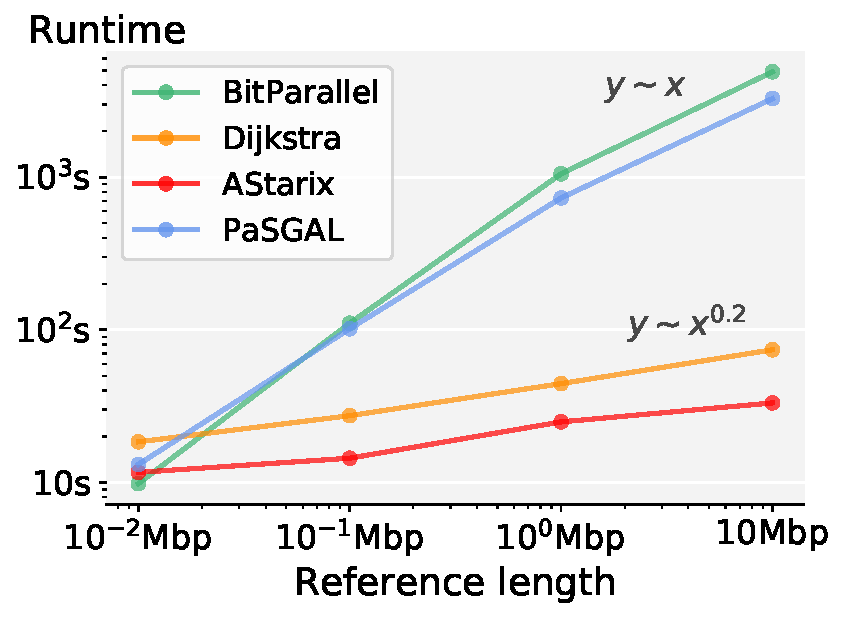
\includegraphics[width=\linewidth]{figs/cmp/performance_vs_genomesize-head_Mbpxs.pdf}
  \end{subfigure}
  \begin{subfigure}{.49\textwidth}
    \centering
    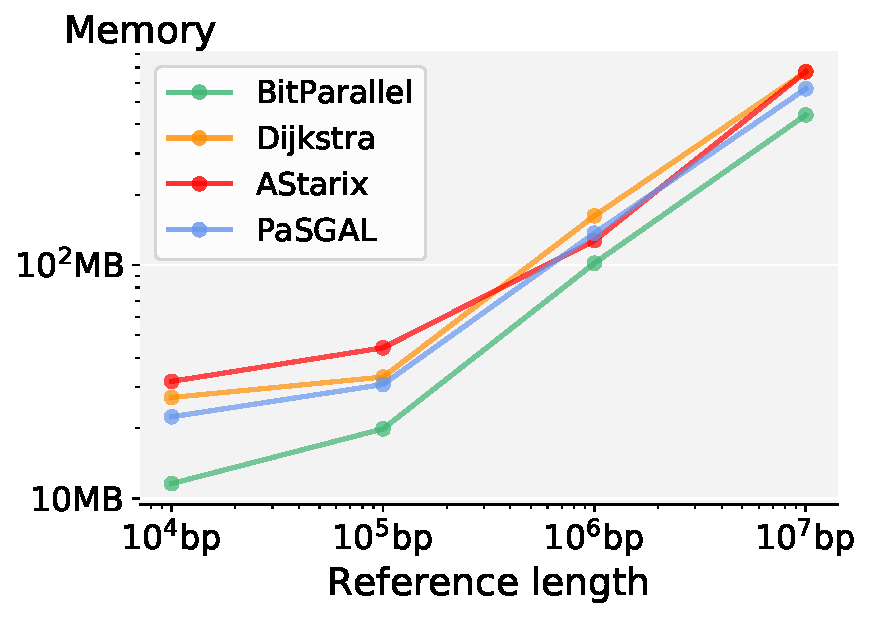
\includegraphics[width=\linewidth]{figs/cmp/memory_vs_genomesize-headxmax_rss.pdf}
  \end{subfigure}
  \caption{Comparison of overall runtime and memory usage of optimal aligners
     with increasing prefixes of E. coli as references.}
  \label{TRIEfig:scaling_with_graphsize}
\end{figure}
